\documentclass[a4paper]{article} 
\usepackage[dutch]{babel}
\usepackage{graphicx}
\usepackage{color}
\usepackage[final]{pdfpages}
\usepackage{hyperref}

\usepackage[margin=3.5cm]{geometry} %ik denk dat de we wel een redelijk aantal paginas gaan hebben wanneer het verslag klaar is, de standaardmarges van latex zijn echt wel groot
%\usepackage[utf8x]{inputenc} 


\title{SWOP - Hospitaal Iteratie 3\\Domain Model and Refactoring Report}
\author{Groep12\\ \\Jeroen Van Gool\\Ruben Lapauw\\Tom De Bie\\Jeroen De Coninck}
\date{}
\pdfinfo{
	/Title (SWOP - Hospitaal Iteratie 2)
	/Author	(Groep 12)
}

\begin{document}
\maketitle
\newpage
\tableofcontents

\section{Problem Domain }

\subsection{Domain Model}

\begin{figure}[h]
\centering
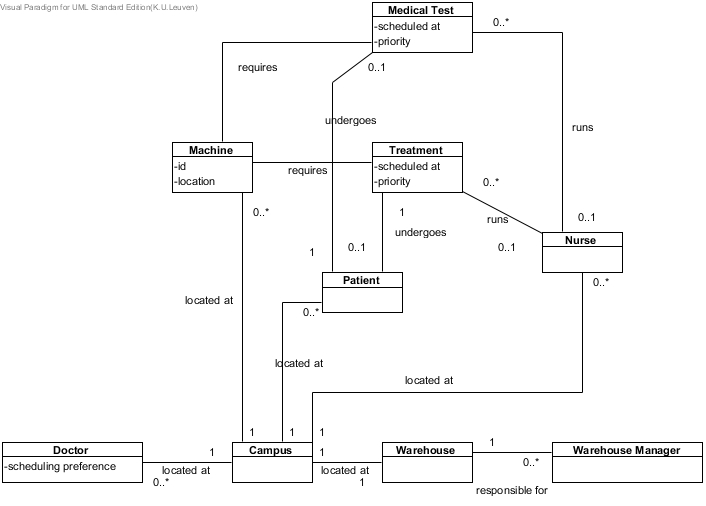
\includegraphics[width=\textwidth]{DomainModel.jpg}
\caption{Domain Model}
\label{fig:domain}
\end{figure}

\subsection{Terminology}

The red text is added in this iteration. Items that didn't change are not in this list.


{\color{red} \textbf{Campus}: a campus is one physical location with its own with its own equipment, warehouse and staff (nurses and warehouse manager).The hospital has two different campuses.}

\textbf{Doctor}: a doctor works at the hospital and is known by his/her name. He is responsible for examining and diagnosing patients when they have an appointment. A doctor orders medical tests,prescribes treatments and is responsible for reviewing medical test and treatment results.{\color{red} A doctor is located at a campus and can have a preference for a campus.}

\textbf{Machine}: every machine in the hospital has a unique identifier and a location. Several types of machines are available. Currently, the available machine types are: X-Ray Scanner, Blood Analyzer, Ultrasound Machine and Surgical Equipment.{\color{red} A machine is located at one campus.}

\textbf{Nurse}: a nurse works at the hospital and is known by her name. She is responsible for registering patients and carries out scheduled medical tests and treatments.{\color{red} A nurse is located at one campus.}

\textbf{Patient}: a patient comes to the hospital with specific complaints, and is known by his/her name.{\color{red} A patient is registered at one campus but can be located at another for medical test.}

\textbf{Appointment}: when registered at the hospital, a patient will have an appointment with a doctor,who will follow the case of the patient. An appointment is scheduled at a certain moment in time, when the doctor is available. An appointment takes 30 minutes to complete.{\color{red} An appointment is located at the campus where the patient is registered.}

\textbf{Medical Test}: a medical test can be used to gather information about the patient's condition. This can be useful both during the diagnostic stage as well as during the treatment stage, e.g. to follow up on certain critical values. A medical test is always carried out by a nurse at the scheduled time.{\color{red} A medical test is carried out at the campus where the machine needed for this test is located. A medical test has a priority.  The scheduling system will take these priorities into account.}

\textbf{Treatment}: a treatment can be ordered by the doctor based on the diagnosis and should lead to the cure of the patient. Treatments are carried out by nurses.{\color{red} A treatment is carried out at the campus where the machine needed for this treatment is located. A treatment has a priority.  The scheduling system will take these priorities into account.}

\textbf{Warehouse}: The stock of the hospital is stored at warehouses inside the hospital.{\color{red} Each campus has one warehouse}. The warehouse can contain:

\textbf{Plaster}: One unit of plaster is used for one cast treatment.

\textbf{Medication items}: The hospital categorizes the medication items it uses as aspirin, vitamins, activated carbon, sleeping tablets, and misc.

\textbf{Meal}: meals are served at 08:00, 12:00, 18:00. We make abstraction of patients unable to eat normal meals. Nurses are not occupied serving meals.

Food and medication items have an expiration date. The hospital is forbidden by law to use food or medication items after its expiration date has passed and throws the food or medication items away at the moment the expiration date passes.
The warehouse has a limited capacity. For easier testability of the system, we set a low capacity: 8 units of plaster, 10 medication items, and 120 meals 4. At startup time, the warehouse is fully stocked.

\textbf{Stock Order}: The hospital places Stock Orders from the Stock Provider to fill in the stock of {\color{red}a} warehouse. For simplicity, we assume an order only contains one type of item, but it can contain a certain amount of items of that same type.

\textbf{Warehouse manager}: A warehouse manager is an employee who unpacks incoming shippings of stock and places it in {\color{red}a} warehouse. He also removes items that have passed their expiration date.



\section{Exceptions}
Het grootste aandachtspunt in de refactoring van ons systeem is het gebruik van Exceptions. We hebben een groot aantal zeer specifieke Exceptions waarvan sommige bijna altijd tesamen voorkomen.
\subsection{Groepering}
De eerste refactoring is dus het groeperen van deze gerelateerde Exceptions onder 1 parent-klasse. Hierdoor wordt de throws-lijst van functies die van deze Exceptions gebruik maken ingekort, met als gevolg dat de code duidelijker wordt.

De Exceptions die deze behandeling krijgen zijn \texttt{ArgumentConstraintException},\\* \texttt{ArgumentIsNullException} en \texttt{ArgumentNotAnsweredException}; deze komen samen onder  \texttt{InvalidArgumentException}. We maken hierbij geen gebruik van Java's ingebouwde \texttt{IllegalArgumentException} omdat deze afgeleid is van \texttt{RuntimeException}, en dit geen gewenst gedrag is. Een tweede groep Exceptions die op deze manier samengenomen worden zijn \texttt{NoSpaceAvailableException} en \texttt{NotEnoughItemsAvailableException}; deze komen onder de parent-klasse \texttt{StockCapacityException}. Deze Exceptions komen normaal niet samen voor maar de omstandigheden waaronder ze voorkomen lijken zodanig op elkaar dat de code eenvoudiger wordt door minder verschillende soorten Exceptions te gebruiken.

Een andere, meer algemene manier om de Exceptions te groeperen is om de Exceptions die minder sterk aan elkaar gerelateerd zijn maar nog steeds bij elkaar horen te groeperen in packages. Hierdoor kan men eenvoudig aan de locatie van een Exception in de package-structuur afleiden waar de oorzaak van de fout vandaan komt. Ook dit hebben we toegepast op ons systeem.

\subsection{Afhandelen}
In de versie van ons systeem die we ingestuurd hebben voor iteratie 2 gaven de meeste functies de verantwoordelijkheid voor het afhandelen van Exceptions door aan de aanroepende code. Dit resulteerde uiteindelijk in functies die zeer veel verschillende Exceptions moesten afhandelen, en deze vaak ook zelf gewoon doorgaven. Uiteindelijk kwamen de Exceptions op een plaats waar ze niet meer konden doorgegeven worden, en omdat het al te laat was om ze nog af te handelen werd er gewoon een \texttt{RuntimeException} gebruikt. In het ergste geval wordt de Exception zelfs niet meer thrown, maar is deze in een aanroepende functie nooit verwijdered, waardoor andere functies die van deze aanroepende functie gebruik maken nog steeds een try-catch clause moeten voorzien voor deze Exceptions.

De refactoring in dit geval is zeer eenvoudig, maar gaat over alle code heen: we handelen elke Exception zo snel mogelijk af, liefst op een plaats waar de fout nog verbeterd kan worden. Het gevolg is dat er doorheen het hele project veel minder Exceptions rondgesmeten worden, en er zeer veel Exception-handling code verwijderd kan worden; een duidelijk vereenvoudiging voor het gebruiken van de code, alswel het aanpassen van de code.

Aangezien deze refactoring zo een grote spanwijdte heeft, is dit nog een work-in-progress. Doorheen de rest van de iteratie zullen we de code doorlopen om dit uit te voeren.

\section{Arguments}
De \texttt{Argument}-klasse is een belangrijke feature van ons systeem die toelaat om op een uniforme manier voorwaarden te stellen op de argumenten die aan verscheidene functies en de signatuur van een functie gelijk te houden voor verschillende child-klassen van een parent-klasse die deze functie moeten implementeren (voornamelijk de \texttt{make}-functie in onze Factories).

Het gebruikt van de \texttt{Argument}-objecten was echter niet al te duidelijk. Hiervoor hebben we de volgende refactorings doorgevoerd:
\begin{itemize}
\item De functie \texttt{getArguments} in \texttt{Factory} dient om de gebruiker te voorzien van een lijst van nog niet ingevulde arguments die compatibel is met \texttt{make} (analoog voor \texttt{Result}). Deze is hernoemd naar \texttt{getEmptyArgumentList} om zijn rol duidelijk te maken.
\item Uit \texttt{make} extracten we een methode \texttt{validate} die controleert of de gegeven lijst van \texttt{Arguments} correct ingevuld is. Dit maakt \texttt{make} duidelijker en verduidelijkt ook weer het gebruik van de \texttt{Argument}-objecten.
\end{itemize}

\section{MachineFactory}
We hebben gemerkt dat de \texttt{make}-functie van al onze \texttt{MachineFactories} hetzelfde zijn op de return-types en aanroep van de relevante constructors van de Machines na dan.

Deze code-duplicatie wordt nu vermeden door het gebruik van de \texttt{validate} functie die we in de vorige sectie beschreven hadden. De duplicate code was namelijk de validatiecode voor de Arguments. Deze kan nu gewoon in de \texttt{validate}-functie van de superklasse geplaatst worden.

\section{Dubbele link Appointment en AppointmentCommand}
Aan het begin van de iteratie had enkel de klasse \texttt{AppointmentCommand} een link naar het bijhorende \texttt{Appointment}-object. Dit bleek echter onvoldoende om preemptive scheduling te implementeren. De scheduler moet immers \texttt{Appointments} die in de weg staan van een andere \texttt{Appointment} met een hogere prioriteit kunnen herschedulen, waarvoor het bijhorende \texttt{AppointmentCommand}-object nodig is.

Om dit op te lossen hebben we de enkele link van \texttt{AppointmentCommand} naar \texttt{Appointment} aangepast naar een symmetrische dubbele link waarmee we vanuit een \texttt{Appointment} ook het bijhorende \texttt{AppointmentCommand} kunnen opvragen.

\section{WorldTime}
De wereld in ons systeem (de klasse \texttt{World}) had met het bijhouden van \texttt{TimeObservers} een verantwoordelijkheid teveel. Om dit recht te zetten hebben we de tijds-gerelateerde functionaliteit van de wereld ge\"{e}xtraheerd naar een aparte klasse: \texttt{WorldTime}.

Deze klasse houdt vanaf nu de tijd en alle {TimeObserver}-gerelateerde functionaliteit die vroeger in de wereld zaten. Hierdoor heeft de wereld geen weet meer te hebben van de \texttt{TimeObservers} en omgekeerd. Een aantal klassen zoals \texttt{Appointment} krijgen dus het \texttt{World}-object niet meer doorgegeven, en kunnen dus ook niet meer aan gegevens die ze niet moesten weten.

\section{Andere refactorings}
\begin{itemize}
\item De klasse \texttt{MedicationArgument} is een klasse die uiteindelijk nergens gebruikt werd, logischerwijs is deze dus verwijderd.
\item \texttt{FoodStock} bevatte een methode \texttt{timeUpdate} die functioneel eenvoudig was, maar onduidelijk geschreven. Deze is herschreven.
\item \texttt{checkValidName} in \texttt{Stock} werd niet meer gebruikt, deze functie is verwijderd.
\item In de klasse \texttt{Warehouse} werd een Warehouse opgezet voor testen, net als met \texttt{World} zetten we dit buiten het echte systeem door deze code in de nieuwe klasse \texttt{BasicWarehouse} te zetten. Hierdoor bevat de \texttt{Warehouse}-klasse geen overbodige code meer en is deze duidelijker.
\item Alle overgebleven \texttt{RuntimeExceptions} worden omgezet naar het gebruik van \texttt{Logger.log()} voor consistentie. Ook dit is een werk van de lange adem dat doorheen de iteratie uitgevoerd zal worden.
\item De \texttt{isValidPosInt}-functie en gelijkaardige functies in \texttt{Utils} worden vervangen door eenvoudige vergelijkingen, dit niveau van indirectie maakte de code niet duidelijker dus kon het beter verwijderd worden.
\end{itemize}

\section{Testen tijdens refactoring}
Onze test suite hebben we gebruikt tijdens het refactoren om ervoor te zorgen dat we de functionaliteit van het systeem niet per ongeluk zouden aanpassen. Hiervoor konden we over het algemeen de test suite gebruiken zoals deze ingeleverd was voor iteratie 2. Daarbovenop konden we ook de nieuw ontwikkelde scenario test suite gebruiken.

In enkele gevallen moest de test suite wel aangepast worden: bij sommige Exceptions, de \texttt{GenericMachineFactory} en de testen die \texttt{Warehouse} gebruikten. Voor deze laatste was de aanpassing eenvoudig: het gebruiken van de nieuwe \texttt{BasicWarehouse}-klasse in plaats van het oude testwarehouse dat opgezet werd door \texttt{Warehouse} zelf.

Voor de Exceptions worden de testen zelfs eenvoudiger: we hebben het aantal Exceptions verminderd, dus moeten de testen ook met minder Exceptions rekening houden. Hier en daar moest er ook gebruik gemaakt worden van de nieuwe parent-exceptions die we ingevoerd hebben in plaats van de individuele child-exceptions.

Tenslotte was het invoeren van de \texttt{GenericMachineFactory} een interface-change, de testen die dus van de vroegere \texttt{MachineFactories} gebruik maakten moesten hier dus voor aangepast worden.

Het gebruik van de testen was vrij eenvoudig: na elke refactoring werden de testen uitgevoerd, indien deze allemaal 'OK' gaven konden we verder naar de volgende refactoring. In het andere geval konden we aan de hand van de gefaalde test(en) uitzoeken wat we aan de werking van het systeem veranderd hadden.
\end{document}
